\documentclass[a4paper,12pt]{article}  % Base font size is set here

% Language setting
\usepackage[british]{babel}

% Set page size and margins
\usepackage[a4paper,top=2cm,bottom=2cm,left=2.5cm,right=2.5cm,marginparwidth=1.75cm]{geometry}

% Use Times font
\usepackage{times}

% Set font size
\usepackage{anyfontsize}
\fontsize{12pt}{14pt}\selectfont

% Packages for additional functionality
\usepackage{float}
\usepackage{graphicx}
\usepackage{parskip}
\usepackage[colorlinks=true, allcolors=black]{hyperref}
\usepackage{amsmath, amsfonts, amssymb}
\usepackage{fancyhdr}


\begin{document}

\pagenumbering{roman}
\begin{titlepage}
  \centering
  \large{\textbf{GHANA COMMUNICATION TECHNOLOGY UNIVERSITY (GCTU) }}\\
  \vspace{0.5cm}
  \large{\textbf{FACULTY OF ENGINEERING}}\\
  \vspace{0.5cm}
  \large{\textbf{DEPARTMENT OF COMPUTER ENGINEERING}}\\
  \vspace{1cm}
  \raisebox{-1.5ex}{
\includegraphics[width=0.6\textwidth]{figures/school_logo.png}}\\
  \vspace{1cm}
  \textit{Topic:}\\
  \vspace{1cm}
  \textbf{AN ENHANCED E-LEARNING PLATFORM FOR AN INTERACTIVE EDUCATIONAL EXPERIENCE}\\
  \vspace{1cm}
  \text{Project Work Submitted in Partial Fulfillment of the Requirements For}\\
  \text{ BSc. in Computer Engineering}\\
  \vspace{1cm}

  \textbf{\textit{BY:}}\\
  \vspace{0.5cm}
  \text{CHRISTIAN NII COMMEY SOLOMON - 040918451}\\
  \vspace{0.5cm}
  \text{JEREMY EDUDZI AVADZI - 4121210061}\\
  \vspace{1cm}
  \textbf{\textit{SUPERVISOR}}\\
  \vspace{0.5cm}
  \text{DR. PHILLIP KISEMBE}\\
  \text{APRIL, 2024}\\
\end{titlepage}
\newpage
\begin{center}
    \section*{DECLARATION}
    This project is submitted as part of the requirements for the BSc. in Computer Engineering awarded by Ghana Communication Technology University. I hereby declare, that this project in its entirety is the result of hard work, research and inquiries. I am confident that this project work has not been copied from another person’s work. All sources of information in this project, have been acknowledged appropriately.
\end{center}

\vspace{1cm}

\subsection*{AUTHORS}
\begin{tabular}{l l}
	\vspace{1cm}
    CHRISTIAN NII COMMEY SOLOMON & SIGNATURE: \underline{\hspace{5cm}} \\
    \vspace{1cm}
    STUDENT ID: 040918451 & DATE: \underline{\hspace{5cm}} \\
    & \\
    \vspace{1cm}
    JEREMY EDUDZI AVADZI & SIGNATURE: \underline{\hspace{5cm}} \\
    STUDENT ID: 4121210061 & DATE: \underline{\hspace{5cm}} \\
\end{tabular}

\vspace{1cm}

\subsection*{SUPERVISOR}
\begin{tabular}{l l}
\vspace{1cm}
    DR. PHILLIP KISEMBE & SIGNATURE: \underline{\hspace{5cm}} \\
    & DATE: \underline{\hspace{5cm}} \\
\end{tabular}

\vspace{1cm}

\subsection*{HEAD OF DEPARTMENT}
\begin{tabular}{l l}
\vspace{1cm}
    DR. SAMUEL DANSO & SIGNATURE: \underline{\hspace{5cm}} \\
    & DATE: \underline{\hspace{5cm}} \\
\end{tabular}
\newpage
\tableofcontents
\newpage
% Switch to Arabic numeral page numbering
\pagenumbering{arabic}
\section{INTRODUCTION}
\subsection{Background of Study}

E-learning is a learning system based on leveraging the capabilities of
technology in teaching and learning practices. It has been on the rise in the
past few years. Many e-learning platforms have been developed to solve problems
that arose due to the pandemic. According to the Ghana Journal of Higher
Education, the modern landscape of higher education is undergoing a shift
towards digital platforms, allowing for a wider accommodation of students
across a relatively broader geographical area for teaching and learning. Amid
the necessities that arose because of the pandemic, e-learning rose to become a
basic form of education at all teaching levels, which actually led to an
increased accessibility and flexibility and also enabled a broader reach for
students across different locations. However, there is the question about the
sustainability of this e-learning trend post-pandemic, and whether there will
be a return to traditional teaching and learning methods, or that the
development of e-learning platforms will be continued by innovators.\\
\vspace{0.2cm}\\ The emergence of e-learning in the traditional teaching and
learning presents its own sets of opportunities and challenges. Gyamfi and Addo
discuss the limitations of the traditional model, especially in addressing the
modern demands of education.\cite{gyamfi2020stakeholders} This approach has struggled to accommodate the
evolving needs of the modern digital age, particularly in providing access to
education, especially in remote regions, contributing to a gap in effective
online learning as compared to traditional learning. They emphasize the
importance of acknowledging the limitations of traditional teaching methods and
embracing innovative approaches to education, such as e-learning. One such
approach would be in the development of a comprehensive, integrated learning
platform that caters to the modern demands of education:- personalize the
learning experience for each student, catering to their individual strengths
and weaknesses; incorporate opportunities for students to develop critical
thinking skills through interactive activities, simulations and project based
learning;developing of digital literacy skills as well as fostering
collaboration and communication among students and tutors.\\ \vspace{0.2cm}\\
There are many such e-learning systems in the world we live in today. Such
platforms like Udemy, ALX SE, Edureka, Scrimba, Harvard Extension, among
others, have played a vital role in facilitating access to educational
resources and opportunities (educational democratization), however, these
platforms often focus on specific niches or cater to a more individual learner
journey.

Kim, Lee \& Yoon \cite{kim2023better}came up with a model to guide the design and development of an
e-learning platform so it would be successful. They suggest five factors that
contribute to the success of an e-learning platform.These are;
\begin{enumerate}
  \item \text{system quality - this is the functionality, reliability and usability of the e-learning platform}
  \item lecture content - referring to the quality, relevance and accessibility of
        learning materials on the platform.\\
  \item teaching quality - which is the effectiveness on the lecturer's part in
        delivering educational content.\\
  \item online interaction - refers to the level of engagement and interaction among
        students, instructors and course materials\\
  \item achievements - which are the tangible outcomes attained by students and
        instructors in relation to predefined learning objectives and performance
        standards that have been set.\\
\end{enumerate}
Despite the comprehensive features offered by platforms like Moodle, which is widely recognized for its flexibility, customization, and robust pedagogical support, it lacks integrated video conferencing capabilities. This limitation is critical for institutions like Ghana Communication Technology University (GCTU), where geographical distance and high costs associated with third-party solutions pose significant challenges. By focusing on these core principles, we aim to create an integrated teaching and learning environment using GCTU as a case study. The internet is the perfect tool for learning, as it offers flexibility and expediency to learners at the same time offering endless opportunities for innovative teaching.

\subsection{Problem Statement}
The goal of this project is to develop a comprehensive, integrated e-learning
platform tailored to the specific needs of universities in Africa, particularly
Ghana Communication Technology University (GCTU). While Moodle, a widely-used
Learning Management System (LMS), offers numerous benefits, it lacks built-in
video conferencing capabilities, which are essential for effective remote
learning. This project aims to address the limitations of current solutions,
enhance accessibility, and reduce costs for GCTU.\\ \vspace{0.2cm}\\ E Learning
provides a very promising solution to this challenges by reducing the reliance
on physical classrooms, thereby enhancing access to education for students in
remote areas and also expand the universities global reach. It will solve the
problem of accommodation constraints by offering courses online, eliminating
the need for everybody to come to campus at once. Also students in remote areas
can access the quality education by using the e-learning platform, regardless
of their location. This bridges the geographical gap and allows for fair and
equal access to quality education. Finally, the university would be able to
extend its wings and offer access to education to students worldwide. Harvard
University’s extension school, for instance, offers a variety of online courses
and even full degree programs to learners worldwide. This move by Harvard,
shows that they recognized the limitations of traditional educational models in
meeting the demands. This would increase the university’s international
recognition and would contribute in creating a global learning community,
whereby students from different countries worldwide can collaborate and learn
together.\\

\subsubsection{Limited Accommodation and Accessibility Challenges at GCTU}
This university faces a significant challenge in providing adequate on-campus
housing for its student population and the ones available around campus are
costly. This results in a large portion of the students body residing far from
campus, often at least 10 kilometers away. This geographical distance creates a
barrier to traditional in-person learning, giving that lectures start at 8 am,
it forces students to make long and potentially expensive and exhausting daily
commutes to attend lectures.\\

\subsubsection{The High Cost of Existing Solutions}
While third-party video conferencing platforms like Zoom or TeamViewer provide
an option for remote learning, the ongoing costs associated with these services
could result in a substantial financial challenge for GCTU. For a technical
institution like GCTU, which encourages innovation and seeks to capitalize on
its own experience, this is particularly concerning. Relying on costly external
solutions is not sustainable in the long term.\\

\subsubsection{The Limitations of Moodle}
Moodle LMS \cite{moodle2024review}, is widely recognized for its flexibility, customization, and robust
features that support various pedagogical approaches. It excels in course
management, user management, communication tools, assessment and grading,
resource management, among other strengths. Despite these strengths, Moodle
lacks a built-in video conferencing feature, which is crucial for facilitating
real-time interaction and collaboration between instructors and students.\\

\subsubsection{The Need for a Custom, Cost-Effective E-Learning Platform}
To address these challenges, GCTU requires a bespoke e-learning platform that
combines the benefits of Moodle with integrated video conferencing
capabilities. This platform must prioritize the following features:\\

\begin{itemize}
  \item i.Video Conferencing: This feature would aim to facilitate real-time
        interaction and collaboration between instructors and students, regardless of
        location, to replicate the traditional classroom experience.\\
  \item Cost-Effectiveness: Eliminating ongoing licensing fees for external video
        conferencing platforms to save valuable resources and ensure long-term
        financial sustainability.\\
  \item Data Privacy and Security: Ensuring full control over student and staff data
        with enhanced security measures tailored to the institution's requirements.\\
\end{itemize}

\subsection{Research Aim and Objectives}
\subsubsection{Research Aim}
The main objective is to develop a web application that facilitates a
high-quality, remote learning experience for students. This platform will
eliminate the need for physical campus attendance by providing a comprehensive
suite of educational tools, including:\\

\begin{itemize}
  \item Video conferencing: To enable real-time interaction between instructors and
        students.\\
  \item Centralized repository: To offer a secure and organized location for accessing
        learning materials such as lectures recordings, notes, assignments.\\
  \item Assessment tools: Allows instructors to evaluate student comprehension through
        various methods such as quizzes, exams, projects.\\
\end{itemize}

\subsubsection{Specific Objectives}
\textbf{Functional Requirements:}
\begin{itemize}
  \item Implement diverse assessment tools (e.g., quizzes, essays, peer reviews)\\
  \item Develop a content management system (CMS) for lecturers\\
  \item Design and develop admin, lecturer, and student interfaces\\
\end{itemize}

\textbf{Non-Functional Requirements:}
\begin{itemize}
  \item Develop a user-friendly interface\\
  \item Ensure robust security measures for data protection\\
  \item Optimize performance for seamless user experience\\
\end{itemize}

\subsection{Significance of study}
The COVID-19 pandemic accelerated the shift towards digital learning, as
highlighted by research conducted by Jakhar et al. (2020). Even though many
schools are trying to transition back to face-to-face or in-person teaching and
learning, the need for having a flexible and accessible learning solution still
remains a priority. In a similar research conducted by the students of GCTU
last year (2023), Adagobo et al,\cite{emmanuel2022design}, proposed that successfully developing a
platform that serves in the context of e-learning would serve the university in
improving learning procedures on campus. Implementing a hybrid approach to
learning, combining the positives of asynchronous learning and synchronous
learning would greatly improve teaching and learning in the school.\cite{islam2015challenges} Students
residing far from campus or juggling work and studies can access course
materials and complete assignments on time, and since some students grasps
concepts quickly, while others benefit from revisiting materials and practicing
at their own pace, the features incorporated on this platform would allow them
to focus on understanding before moving on. Some students also prefer visual
learning through recordings, while others benefit from interactive activities.
This hybrid approach would cater to these different learning styles.\\

\subsection{Scope and Limitation}
\subsubsection{The scope of this research}
This research will focus on developing a comprehensive online learning module
as a pilot program for the Computer Engineering and Telecommunications
Engineering Program within the Faculty of Engineering at Ghana Communication
Technology University. The platform will be designed with scalability in mind
to accommodate future integration with other faculties in subsequent
iterations.\\

\subsubsection{The limitations of this research}
\begin{enumerate}
  \item The initial development phase will prioritize core functionalities like video
        conferencing, content delivery, and assessment tools.
  \item The pilot program will be implemented with courses offered by the Faculty of
        Engineering. Scaling the platform university-wide will require additional
        planning and resource allocation to accommodate the needs of other faculties.
  \item External factors such as unreliable internet connectivity and power supply in
        some regions of Ghana could potentially impact the platform's effectiveness.
        Future research directions could explore incorporating offline functionalities
        or developing partnerships with internet service providers to address these
        challenges.
\end{enumerate}

\subsection{Brief Methodology}
\subsubsection{ Design Concept}
This project will implement an Agile development approach using the Scrum
framework. Scrum places a strong emphasis on user feedback, iterative
development, and continuous improvement.\\

\begin{enumerate}
  \item Product Backlog: A comprehensive list of functionalities will be created,
        prioritizing features based on user needs and project goals.\\
  \item Sprints: Development will occur in short, time-boxed sprints (2-week
        iterations) where a set of features is developed, tested, and deployed.\\
  \item User Feedback: After each sprint, user feedback will be incorporated to refine
        the platform and prioritize features for future iterations.\\
\end{enumerate}

This approach allows for flexibility and adaptation as the project progresses,
ensuring the final platform effectively meets the needs of students,
instructors, and administrators.\\

\begin{figure}[H]
  \centering
  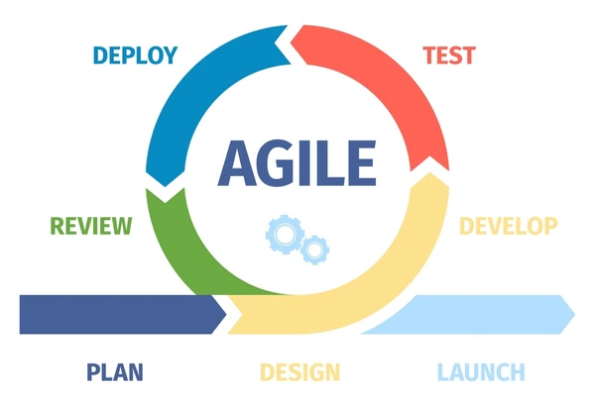
\includegraphics[width=1\textwidth]{figures/agile.png}
  \label{fig:1.6.0}
  \caption{The Agile Software Development Module}
\end{figure}

\subsubsection{Software required}
i.Microsoft Windows 10 Home or 11 Home\\ ii.Visual Studio Code for Windows \\
iii.Chrome, Firefox Web Browsers\\

\subsubsection{Frameworks and Libraries}
i.MongoDB Atlas for hosting our MongoDB database\\ ii.NodeJS to serve as the
runtime environment for our server\\ iii.ExpressJS as our web Framework\\
iv.HTML, CSS and JavaScript for our client side development.\\ v.Socket.io for
real-time bidirectional communication\\ vi.Git and GitHub for version control\\

\subsubsection{Hardware Requirements}
i.Processor (CPU):\\ Minimum: Intel Core i5-8th Gen or AMD Ryzen 5 3rd Gen (or
equivalent)\\ Recommended: Intel Core i7-10th Gen or AMD Ryzen 7 3rd Gen (or
equivalent)\\ ii.RAM: \\ Minimum: 8GB DDR4 RAM\\ Recommended: 16GB DDR4 RAM -
This would allow us to run multiple development tools smoothly\\ iii.Storage:\\
Minimum: 256GB SSD for faster loading times and overall performance\\

\subsection{Organization of Project}

The project is organized as follows: Chapter 1 covers the introduction, study
background, issue description, major and secondary objectives, significance of
the study, scope and limitations, process, and project organization. In Chapter
2, the literature review is discussed in order to offer an analysis of relevant
and current research studies. The project's methodology is thoroughly discussed
in Chapter 3. This is an extended version of the brief method from chapter 1.
Chapter 4 covers outcomes and analysis, or the evaluation and analysis of
results. Chapter 5 is meant to be the conclusion.\\ \newpage

\section{LITERATURE REVIEW}
\subsection{Overview}
This chapter conducts a comprehensive review of the existing literature
relevant to the field of study. It lays the foundation for the proposed project
by by providing a detail analysis of each of the projects parts. This chapter
explores the theoretical frameworks and methodological approaches used in
earlier studies. It offers an evaluation of of relevant projects pertaining to
WebRTC (Web Real Time Communication), SSR (Server Side Rendering), Scalable
Database management Systems and the use of ODM (Object Data Modelling)
libraries, Containerization, System architecture design to avoid SPOF (Single
Point of Failure) as well as Web Sockets. Reviews in this chapter are drawn
from online resources and journal publications.\\

\subsection{Current Issues of Concern}
The university system in Ghana is having a hard time keeping up with the
increasing number of students enrolled. The restricted housing options on and
around campus leads to bottlenecks, and students in remote locations frequently
do not have access to high-quality educational programs. Universities also find
it difficult to have a solid worldwide reputation and reach outside of Ghana.
These problems undermine both the overall influence of Ghanaian institutions
and educational equity. Furthermore, the increasing demand for flexible and
accessible learning options adds another layer of complexity. Students are
looking for educational options that work with their hectic schedules and
geographic constraints. This increasing demand for flexibility may not be met
by traditional classroom environments.\\

\subsection{Definition of Related Areas}
This section reviews detailed definitions that are closely related to the
project topic and scope, aiming to make things clearer and further
understanding of the project.\\

\subsubsection{WebRTC (Web Real Time Communication)}
WebRTC, which stands for Web Real-Time Communication, empowers peer-to-peer
associations without the require for third-party servers.Information sharing
over WebRTC is straightforward, supported by WebRTC APIs, and accessible at
many stages thanks to its simplicity. At first, servers are required for
clients to set up associations. After the initial setup, clients can talk
directly to each other, without the server involved.When a client sends data to
the signaling server, the server transfers this data to the other client. After
accepting this information, the client stores it locally. In this way, this
client sends its claim information to the server, which transfers it to the
other client. This trade guarantees both clients are mindful of each other,
encouraging an association foundation. Signaling servers, utilized for this
information trade, are standard servers with the sole reason of encouraging
client information trade.\cite{emmanuel2022design} The method of exchanging information from one client
to another in WebRTC is called signaling. In WebRTC session establishment, the
initial step is offer generation. A client initiating communication creates an
offer, typically a JavaScript object encapsulating Session Description Protocol
(SDP) data. The Session Description Protocol (SDP) embedded within the offer
specifies media capabilities, such as video and audio codecs supported. The
client sends this offer to the signaling server, which forwards it to the other
client. Upon receiving the offer, the other client stores it locally and
constructs an answer containing its own SDP information. This answer, also
transmitted via the signaling server, details the recipient's media
capabilities. While both parties now possess a mutual understanding of each
other's media offerings, an additional exchange of data, termed ICE
(Interactivity Connection Establishment) candidates, is necessary to establish
the peer-to-peer connection. Clients give URLs of these servers to the WebRTC
API to get ICE candidates. As the client makes an offer, ICE candidates are
recovered from the servers. These candidates are at that point sent to the
other client by means of the signaling server. The same handle happens when
creating answers. Once both clients have each other's SDP information and ICE
candidates, they can build up a coordinate peer-to-peer association.
Information transmission through WebRTC APIs from that point happens
straightforward between the clients, empowering efficient and secure real-time
communication.\\

\subsubsection{Web Sockets}
Web Sockets allow for two way communication, between a client like a web
browser and a server through a persistent, full-duplex connection. Unlike HTTP
requests where the client typically initiates communication and the connection
closes after each response, Web Sockets remain open, allowing both the client
and server to exchange messages at any time. This back and forth communication
is ideal for applications requiring low latency real time updates, such as chat
platforms, online games or collaborative editing tools. By using a handshake
process HTTP upgrade request and Web Socket Handshake to establish
connections, Web Sockets can efficiently receive data in both directions
without the need for repeated setup. This efficiency makes Web Sockets more
effective for real time communication compared to methods like polling or long
polling. In summary Web Sockets offer a solution, for creating web applications
that demand immediate responsiveness and minimal delays.\\

\subsubsection{Server Side Rendering}
Server-side rendering (SSR) is a procedure that renders a web page on the
server instead of within the browser. When a website is rendered on the server,
a completely rendered page is sent to the client and the client's JavaScript
bundle locks in and empowers the Single Page Application system to function.
Server side rendering (SSR) is a method employed in web development where the
server dynamically creates the HTML content of a web-page and sends it to the
clients browser. This differs from client side rendering, where the browser
uses JavaScript to generate the HTML content after receiving HTML from the
server.In SSR, when a user asks for a web page, the server handles the request,
collects the data from a database or external APIs, and then generates the HTML
content incorporating this data. The entire HTML page is then transmitted to
the client's browser for display without any processing. This approach can lead
to quicker initial page loading times. Improved search engine optimization
(SEO) since search engines can easily scan and index the HTML content. SSR is
frequently utilized in web applications developed with server side technologies
like Node.js, Django, Ruby on Rails and PHP. It proves advantageous for
websites with content or dynamically generated content where SEO and
performance play vital roles. Nonetheless implementing SSR may add complexity
to development and up keep efforts as it necessitates handling of server side
and client side logic to ensure consistency and optimal performance, across
platforms and devices.\\

\subsubsection{Success of  e-learning  platforms}
The rise of online learning platforms can be explained by several key factors.
First, their on-demand access model grants learners anytime, anywhere learning,
enabling them to progress at their own pace. Second, eLearning platforms offer
a varied content library, catering to various learning preferences through
multimedia elements like quizzes, interactive videos, and simulations. These
elements promote increased learner engagement and improve knowledge retention.
Finally, the inherent scalability and adaptability of eLearning platforms allow
them to effectively serve a wide range of learners with diverse learning needs.
Research conduction by S.Kim et al(2015)\cite{kim2023better} suggests that five core principles
significantly contribute to the success of an eLearning platform:\\

\begin{enumerate}
  \item System Quality: This encompasses the platform's technical functionality,
        reliability, and user-friendliness. Here, factors like intuitive interface
        design, responsiveness, and seamless content delivery are crucial.\\
  \item Content Quality: This refers to the quality, relevance, and accessibility of
        learning materials hosted on the platform. Content should be well-organized,
        current, and aligned with established learning objectives.\\
  \item Instructional Design: This focuses on the effectiveness of the instructional
        methods employed in delivering the learning content. This includes factors like
        clear learning objectives, well-structured content delivery, and the use of
        appropriate pedagogical approaches.\\
  \item Online Interaction: This emphasizes the level of engagement and interaction
        within the platform. This includes fostering communication and collaboration
        among learners, instructors, and the learning materials themselves through
        discussion forums, group activities, and interactive assessments.\\
  \item Learning Outcomes Assessment: This refers to the process of measuring and
        evaluating the knowledge and skills acquired by learners against predefined
        learning objectives and performance standards. Effective assessment strategies
        should be integrated within the platform to track learner progress and provide
        feedback for continuous improvement.\\

        By focusing on these core principles, eLearning platforms can create an
        integrated and learner-centric teaching and learning environment.
\end{enumerate}

\subsubsection{Scalable No-SQL Database Management Systems}
MongoDB stands out as a liked No-SQL database recognized for its ability to
scale effectively. Its distributed architecture is the key, to this scalability
allowing it to manage data volumes and heavy traffic loads efficiently. MongoDB
utilizes sharing to distribute data among servers facilitating scaling. This
implies that as data and traffic increase you can expand the number of servers
in the MongoDB cluster to accommodate the growing demand. The adaptability of
MongoDB schema also plays a role in its scalability. Unlike databases MongoDB
does not mandate a predefined schema making it simple to introduce new fields
or modify existing ones without any downtime. This adaptability proves
beneficial in environments where requirements are subject to frequent changes.
Apart from scaling MongoDB also supports scaling by enabling you to enhance
individual server resources (such as CPU and RAM) within the cluster to manage
higher workloads. The combination of vertical scaling capabilities makes
MongoDB a scalable database solution suitable for various applications ranging
from small startups, to large enterprises.\\

\subsubsection{Containerization with Docker }
Docker, an example of containerization transforms the landscape of software
development and deployment by packaging applications and their requirements,
into self contained units known as containers. These containers operate
reliably across settings spanning from development, to production guaranteeing
behavior of applications regardless of their deployment location.
Containerization offers application segregation, flexibility and optimized
resource usage simplifying the development and deployment workflow while
enhancing resource efficiency compared to machines.\\

\subsubsection{System Architecture Design avoiding Single Point of Failure}
A critical aspect of system architecture design is the elimination or
mitigation of Single Points of Failure (SPOFs). An SPOF is a single component
whose failure can cause the entire system to become inoperable. It's really
important to make sure that a our system doesn't rely on one part that could
cause the whole thing to fail. When a single point of failure occurs it means
that if one component breaks the entire system will stop working. To prevent
this, methods like having backups and being able to handle faults are used to
keep the system running even if something goes wrong with one or more parts.
This is particularly crucial, in systems where any downtime could lead to
losses or affect how users interact with it. Ultimately avoiding points of
failure helps boost the reliability, availability and resilience of a system.\\

\newpage
\subsection{REVIEW OF RELATED AREAS}
This section provides an overview of other studies done by other authors that
are relevant to this work. It briefly outlines the working of the systems
examined in these related works, along with the methodologies used by the
respective authors. Furthermore, it evaluates the strengths and weaknesses in
these related works.\\

\subsubsection{1 Reviewed Work One}
\large\textbf{Review of Moodle LMS}\\

This review of Moodle explores the existing research and academic discourse
surrounding its development, implementation, and impact in educational
settings. This review typically examines various aspects such as its
effectiveness as a learning management system (LMS), pedagogical benefits,
challenges, and user perceptions.\\

\textbf{1.Effectiveness as an LMS}\\
Moodle is widely recognized for its flexibility and customization options, allowing educators to tailor the learning environment to specific needs (Al-Ajlan \& Zedan, 2008). Some Studies highlight its effectiveness in enhancing student engagement and interaction through forums, quizzes, and collaborative tools (Brandl, 2005). Other studies often show Moodle performing favorably against other LMS platforms in terms of user satisfaction and feature richness (Machado \& Tao, 2007).\\

\textbf{2.Pedagogical Benefits}\\
Dougiamas suggests Moodle enables active learning, collaboration, and self-paced study. The platform's tools, such as workshops and wikis, facilitate peer assessment and collaborative learning, fostering a deeper understanding of course material and the integration of  multimedia resources and interactive activities in Moodle courses has been shown to improve knowledge retention and comprehension.\\

\textbf{3.User perceptions and Experiences}\\
Students generally report a positive experience with Moodle, appreciating its accessibility and the ability to review materials at their own pace. Also being able to submit assignments, partake in quizzes and live discussions. However, continuous professional development and support are crucial for maximaizing the platform’s potential and ensuring effective usage. (Ullman \& Rabinowitz 2021).\\

\textbf{4.Challenges and Limitations}\\
Currently, Moodle primarily supplements traditional face-to-face classroom pedagogical methods. However, the imperative to transition fully to remote learning is increasingly critical. It's essential to define the learning context within the institution based on the capabilities and functionalities that the platform offers. This shift necessitates leveraging Moodle beyond its current supportive role to establish a comprehensive framework for remote education, addressing both technical and pedagogical challenges to enhance the institution's educational delivery and adaptability to modern learning environments.\\

\subsubsection{ Reviewed work two}
\large\textbf{The Process of Designing the Functionalities of an Online Learning Platform- A Case Study By; (Robert Oliwa, 2021)}\\

In this study, the author is looking into the process of designing the
functionalities of an online learning platform as proposed by three distinct
user groups: students, academics, and administrative staff. Furthermore, the
study aims to acquire insight into how these participants' opinions influence
the platform construction process. Using a case study design, the author
investigates whether users of the online learning platform can help define its
functionalities, specifically remote class creation and sharing, test
administration, and enhanced student activity reporting. Within the context of
Ghana Communications Technology University, by involving students, instructors,
and administrative staff in platform development, the proposed e-learning
platform for GCTU can address diverse needs and preferences, ensuring
accessibility, flexibility, and cost-effectiveness.\cite{oliwa2021process} \\

\textbf{Methodology}\\
The study used a mixed-methods approach to assess the design and functionality of an online learning platform through the eyes of students, professors, and administrative staff.\\

\textbf{Qualitative Data Collection}\\
Individual interviews were held with randomly selected individuals from each user group (students, teachers, and administrative personnel). These interviews provided detailed insights into participants' preferences, experiences, and needs for the online learning platform. Questions that were open-ended allowed participants to freely express their ideas and suggestions, leading to an even more specific understanding of their perspectives.\\

\textbf{Quantitative Data Collection}\\
A detailed online survey was distributed to a handful of students and teachers to get quantitative data on their thoughts and experiences with the online learning platform's functions or what said functions should be. The survey used structured questions and Likert scales to quantitatively assess participants' attitudes and preferences. This enabled a systematic examination of replies and the discovery of trends and patterns across various user groups. This study has established grounds for the development of a successful e-learning platform by employing a mixed-methods approach.\\

\textbf{Strengths of study}\\
1.By combining qualitative feedback from individual interviews with quantitative data from surveys, the study gathered a wide spectrum of viewpoints from students, teachers, and administrative personnel. \\
2.The integration of qualitative and quantitative data enabled a comprehensive synthesis of findings, resulting in useful suggestions for improving the design and effectiveness of an online educational platform.\\

\textbf{Limitations of the study}
1.The study sample size which was used might have been limited which would mean that the conclusions drawn from the study cannot be applicable in a more generalized setting or outside the context of the research.

\subsubsection{ Reviewed Work 3}
\large\textbf{Design And Implementation Of A Desktop Based System To Enhance Teaching Using Screen Sharing Technology Through Wlan Using GCTU As A Case Study( Adabogo Emmanuel,  Gertrude Fafali, 2022)}\\

This study aims to address several key challenges and to improve the overall
learning experience for both lecturers and students. Their approach aimed to
allow for seamless sharing of educational materials, presentations to eliminate
the need for costly subscription-based virtual classrooms. Using real-time
video and audio sharing mechanisms with WebRTC, they aimed to optimize the
platform to allow for interactive discussions and collaborations between
lecturers.\cite{emmanuel2022design}\\

\textbf{Methodology}\\
The methodology that the authors employed encompasses several key components aimed at designing and implementing a screen-sharing software for e-learning purposes.\\

\begin{enumerate}
  \item Technology Selection: The study begins by carefully identifying appropriate
        technologies for designing and implementing the screen-sharing system. This
        phase considers factors like efficiency, tolerance for errors, scalability, and
        cost efficiency.\\
  \item WebRTC Implementation: They utilize WebRTC to facilitate real-time
        communication and data transfer between lecturers and students. This technology
        provides a framework for audio and video peer to peer streaming over the web
        without the need for a third party, making it ideal for this application.\\
  \item Back-end Development: The utilized JavaScript runtime, NodeJS for the back-end
        development, which is responsible for the server-side operations.\\
  \item User interface design: They used HTML and CSS from the front-end or user
        interface, which is the part of the application that users interact with.\\
  \item Scalability Assessment: The system's scalability is assessed, taking into
        account elements such as the number of concurrent users it can support and its
        ability to handle increasing workload demands.\\
\end{enumerate}

\textbf{Strengths }\\
\begin{enumerate}
  \item By utilizing WebRTC technology and implementing real-time screen sharing
        capabilities, the study offers an innovative solution to address the challenges
        faced in traditional e-learning environments.\\
  \item The research's focus on building a desktop-based system with open-source
        technologies such as JavaScript, HTML, and CSS shows its focus on
        cost-effectiveness. The study offers universities a more financially
        sustainable alternative to pricey subscription-based virtual classroom
        applications.\\
  \item Along with basic screen-sharing capabilities, the system supports chat,
        file-sharing, and audio streaming. These extra features improve the e-learning
        experience by encouraging interaction and collaboration between lecturers and
        students in virtual classroom environments.\\
  \item The system's design prioritizes scalability, with up to 26 individuals using a
        single 4G WIFI interface. This scalability means that the system can
        effectively serve different class sizes while also adapting to the changing
        needs of educational institutions throughout time.\\
\end{enumerate}

\textbf{Limitations }\\
\begin{enumerate}
  \item The study focuses primarily on the development and testing of a screen-sharing
        system that employs WebRTC technology. It may not include all aspects of
        e-learning, including assessment methodologies, curriculum design, and learner
        engagement strategies.\\
  \item While the system has effective screen-sharing features, it may have technical
        restrictions such as bandwidth, latency, and device compatibility. Users with
        slower internet connections or older technology may have performance issues,
        which limit the system's accessibility and usability.\\
  \item The findings of the study may be specific to the context in which it was
        conducted, such as the particular technological infrastructure and user
        preferences within the university campus; drawing the results to other
        educational settings or cultural contexts might require additional change.\\
\end{enumerate}

\subsubsection{ Reviewed Work 4}
\large\textbf{Design and Implementation of Online-Learning platform with a large class size:
  Case study at University of Energy and Natural Resources-Ghana By; ( Peter
  Appiahene, Christopher Ninfaakang, 2017)}\\

This research explores the experimental use of a web-based platform to
supplement and improve the teaching and learning of the Computer Literacy and
Information Technology course at Ghana's University of Energy and Natural
Resources (UENR103). The study was conducted over two academic years with a
combined class of over 300 students each year. The document discusses the
methodology used in developing the online-learning platform, the results of
implementing the platform, student engagement through activities like group
discussions and self-assessment tests, and the overall response from students
and instructors to the technology-supported learning environment. The study
aims to showcase the application of online learning for large classes and how
it was implemented at the University of Energy and Natural Resources, providing
insights into the benefits and challenges of using technology in education.\cite{appiahene2017design}\\

\textbf{Methodology }\\
The first phase of the study focused on developing a web-based
platform tailored to supplement the teaching and learning of the Computer
Literacy and Information Technology course at the University of Energy and
Natural Resources (UENR). This involved collaboration between instructional
designers, web developers, and subject matter experts to create a platform that
aligns with course objectives and student needs. The developed online-learning
platform was implemented over two academic years, accommodating a combined
class of over 300 students each year. This phase involved integrating the
platform into the course curriculum, providing access to students, and
facilitating instructor training on platform usage and management. Throughout
the study, student engagement was promoted through a variety of activities
supported by the online learning platform. These activities included group
discussions, self-evaluation assessments, interactive quizzes, multimedia
information delivery, and collaborative projects. The goal was to encourage
active learning, involvement, and knowledge retention among students.\\

\textbf{Strengths }\\
\begin{enumerate}
  \item Providing the option for students to read materials or watch videos caters to
        diverse learning styles and preferences, accommodating different ways in which
        students may absorb information effectively.\\
  \item The ability for students to submit assignments online and download materials
        from the platform streamlines the process of academic tasks, making it more
        convenient and efficient for both students and faculty.\\
  \item The implementation and testing phase of the project highlight the main features
        of the e-learning system, such as authentication mechanisms, database
        utilization, user account management, and error handling, indicating a
        comprehensive and well-thought-out development process.\\
\end{enumerate}

\textbf{Limitations}\\
The authors faced challenges in gathering information and data from
users for an objective assessment of the proposed e-learning products was
challenging. Expected users were unwilling to provide input or gave vague
information, leading to uncertain results.\\

\subsection{SUMMARY OF RELATED WORKS}
The reviewed literature highlights various aspects of e-learning platforms,
each with its strengths and limitations. The first review of Moodle LMS
underscores its flexibility and customization, effective student engagement,
and positive user perceptions, despite challenges in fully transitioning to
remote learning. The second work, a case study on designing functionalities for
an online learning platform, emphasizes the value of user input in platform
development, with a mixed-methods approach revealing insights into user
preferences and the importance of accessibility and flexibility. The third
review discusses a desktop-based screen-sharing system using WebRTC,
highlighting its cost-effectiveness, real-time interaction capabilities, and
scalability, although it may face technical limitations and context-specific
challenges. Lastly, the fourth review examines an online learning platform for
large classes at the University of Energy and Natural Resources, showcasing its
benefits in enhancing student engagement through diverse activities, while
noting the difficulty in gathering comprehensive user feedback for objective
assessment. Together, these works provide a comprehensive understanding of the
design, implementation, and impact of various e-learning systems, emphasizing
the importance of user-centered design, technological adaptability, and
continuous improvement to address the evolving needs of educational
environments.\\

\subsection{IDENTIFED GAPS FROM THE RELATED WORKS}
From the weaknesses identified in the four reviewed works, the following gaps
were identified:\\

\begin{enumerate}
  \item Limited Remote Learning Capabilities: Although Moodle and other platforms
        provide robust support for blended learning, there is an insufficient focus on
        fully remote learning environments. The transition to comprehensive online
        learning is hindered by inadequate leveraging of existing tools and features to
        support remote education effectively.\\

  \item User Involvement in Design: While the case study on designing online learning
        platform functionalities emphasizes user input, many platforms still lack
        significant engagement from students, instructors, and administrative staff in
        the design process. This limits the platform's ability to fully meet the
        diverse needs of its users.\\

  \item Technical Limitations in Real-Time Interaction: The desktop-based
        screen-sharing system using WebRTC offers innovative solutions for e-learning,
        but it does not comprehensively address issues related to bandwidth, latency,
        and device compatibility. These technical limitations affect the overall
        accessibility and performance of the system.\\

  \item Scalability and Performance: The online learning platform for large classes at
        the University of Energy and Natural Resources demonstrates the challenges of
        scaling e-learning systems. There is a need for solutions that can handle
        larger class sizes without compromising performance, ensuring seamless access
        for all students.\\

  \item Comprehensive Feature Integration: Many existing e-learning platforms do not
        fully integrate essential features such as audio transmission, real-time video
        conferencing, and collaborative tools. This results in a fragmented learning
        experience that can impede effective communication and interaction among
        users.\\
\end{enumerate}

\subsection{CURRENT SETUP OF E-LEARNING PLATFORMS}
\begin{figure}[H]
  \centering
  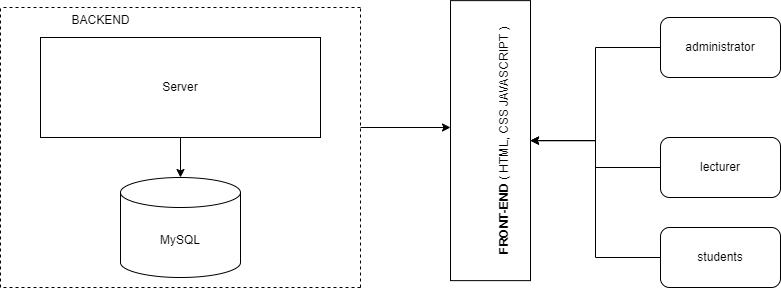
\includegraphics[width=1\textwidth]{figures/current.png}
  \caption{The current setup of e-learning systems (P. Appiahene et al, 2017)\cite{appiahene2017design}}
\end{figure}
The current setup of e-learning systems, as depicted in the provided diagram,
functions primarily as a drop box for resources, allowing users to access
content. Here's a detailed explanation:\\
\large\textbf{Backend}\\
\textbf{Server:} The server is the central component of the backend infrastructure. It
handles all the requests from the front-end and processes them. It is
responsible for managing the flow of data between the front-end and the
database.\\

\textbf{MySQL Database:} The MySQL database stores all the data related to the
e-learning system. This includes user information (administrators, lecturers,
students), course materials, assignments, and other educational resources. The
server interacts with the database to retrieve, store, and manage data.\\

\large\textbf{Front-End}\\
\textbf{Technologies Used:} The front-end of the system is built using HTML, CSS, and
JavaScript. These technologies are used to create the user interface that the
administrators, lecturers, and students interact with.\\

\large\textbf{User Roles}\\
\textbf{Administrator:} Administrators manage the overall system. They have access to
add, update, and delete resources, manage user accounts, and perform other
administrative tasks. They ensure that the system runs smoothly and
efficiently.\\

\textbf{Lecturer: }Lecturers can upload and manage course materials, assignments, and
other educational content. They interact with the system to provide resources
to students and possibly to receive assignments or tests from them.\\

\textbf{Students: }Students primarily use the system to access the educational content
uploaded by lecturers. They can download materials, view lectures, submit
assignments, and possibly take quizzes or exams if such features are
integrated.\\

\large\textbf{Functionality}\\
The current e-learning system setup is essentially a repository for educational
resources. It provides a centralized location where various users
(administrators, lecturers, and students) can interact with the system
according to their roles.\\

\textbf{Resource Upload and Management:} Lecturers and administrators can upload and
manage resources such as lecture notes, assignments, and multimedia content.\\
\textbf{Resource Access:} Students can access and download these resources, facilitating
their learning process.\\

\subsection{PROPOSED DESIGN OF E-LEARNING PLATFORM}
Our proposed e-learning solution is designed to provide a highly interactive
and efficient learning environment through the integration of advanced
technologies. At the core of our platform, we will leverage WebRTC to enable
real-time video conferencing, ensuring that live lectures and interactions are
smooth and responsive. For the back-end infrastructure, we will utilize the
Express web framework within the Node.js runtime, which will offer a scalable
and performant server-side solution. To manage and store data efficiently, we
will employ MongoDB, a NoSQL document-based database management system known
for its scalability and flexibility. This hybrid architecture is strategically
chosen to deliver a seamless performance and an optimal user experience across
a wide range of devices and varying network conditions, ensuring that our
e-learning platform is both robust and adaptable.\\

When selecting technologies for designing and implementing this system, it is crucial to consider factors such as efficiency, fault tolerance, flexibility, and reusability. Additionally, evaluating time and cost effectiveness, user-friendliness, appealing interfaces, future maintenance needs, and overall performance is essential.\\

\begin{figure}[H]
  \centering
  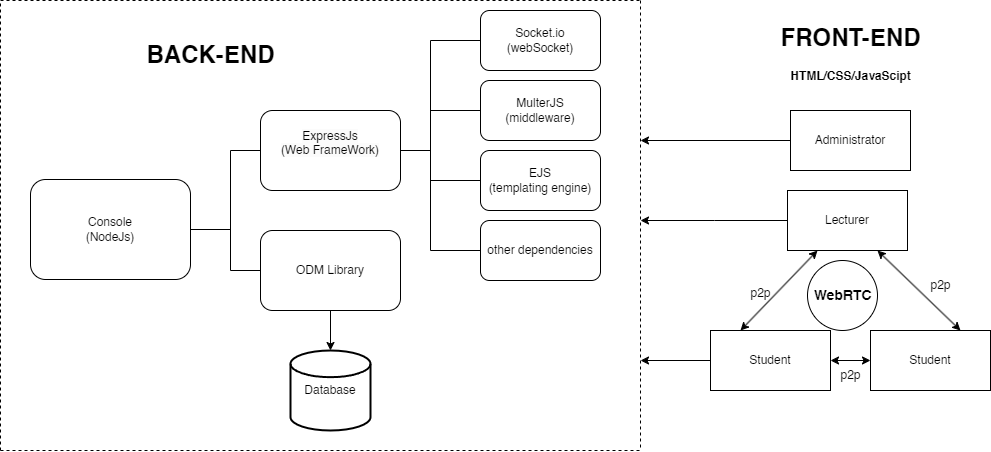
\includegraphics[width=1\textwidth]{figures/proposed.png}
  \caption{Our Porposed design of the E-learning platform}
\end{figure}

\subsection{CONCLUSION}
In conclusion, the literature review emphasises the important factors and developments required for creating a successful e-learning platform. The suggested solution claims to provide a robust, adaptable, and user-centric educational experience by using WebRTC for real-time video conferencing, using the Express framework on Node.js for the backend, and utilising MongoDB for scalable data management. Emphasising elements like efficiency, fault tolerance, and cost efficiency guarantees that the platform meets current technological expectations while being adaptive to future improvements. This complete strategy not only meets the immediate needs of smooth performance and user engagement, but also positions the platform for long-term success and growth in the ever-changing field of digital education.\\
\newpage

\bibliographystyle{IEEEtran}
\bibliography{references.bib}

\end{document}